\section{Experiments}
\tk{order: CLEVR + baselines without TL, COG + baseline without TL, Feature Transfer-CLEVR/CoGenT, Temporal Transfer - COG, Reasoning Transfer - CLEVR/CoGenT, Reasoning Transfer-COG}

\newpage
\subsection{CLEVR/CoGenT dataset: baseline comparison}

\tk{description of CLEVR and CoGenT datasets, task families/groups}

\begin{table}[ht]
	\centering
	%\begin{adjustbox}{width=0.45\textwidth}
	\begin{tabular}{cccc}
		\toprule
		Dataset	& Cubes	& Cylinders &	Spheres	\\
		\midrule
		CoGenT A &  Family A  & Family B 	&	Any color  \\
		CoGenT B	&	Family B  &	Family A	&	Any color \\
		\bottomrule
	\end{tabular}
	%\end{adjustbox}
	\caption{Restrictions on feature combinations in A \& B conditions of the CoGenT variant of the CLEVR dataset.}
	\label{tab:cogent_conditions}
\end{table}


\tk{comparison of our model with selected baselines - pure CLEVR? (or CoGenT?), no transfer learning}

\tk{figure(s) with accuracy on CLEVR/CoGenT is/are missing!}

\begin{figure*}[htbp]
	\centering
	\begin{subfigure}{\textwidth}
		\centering
		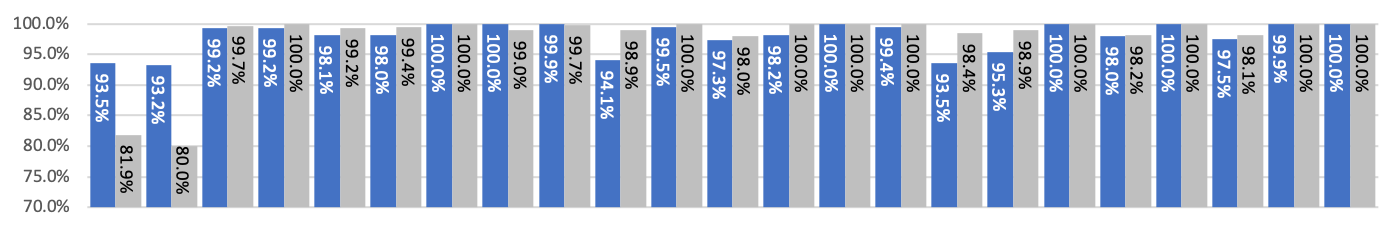
\includegraphics[width=0.9\textwidth]{../results/samnet_cog_orig_canonical_no_labels.png}
	\end{subfigure}%
	\newline
	\begin{subfigure}{\textwidth}
		\centering
		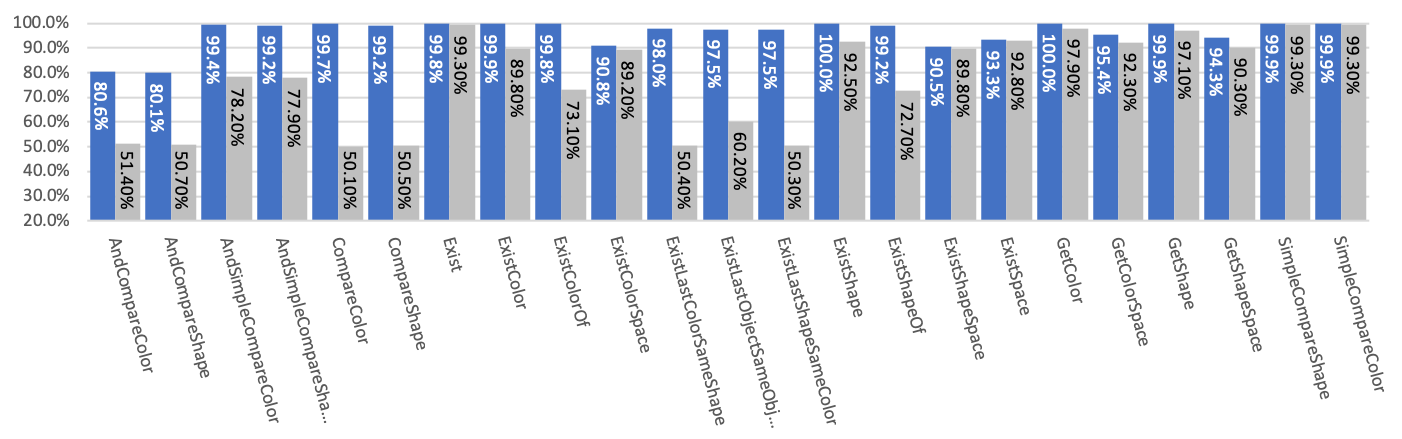
\includegraphics[width=0.9\textwidth]{../results/samnet_cog_orig_hard.png}
	\end{subfigure}%
	\caption{Comparison of test set accuracies of SAMNet (blue) with original results achieved by the 
		baseline model~\cite{yang2018dataset} (gray) on Canonical (top) and Hard (bottom) variants of the COG dataset.}
	\label{fig:samnet_cog_detailed}
\end{figure*}

\newpage
\subsection{COG dataset: baseline comparison}

\tk{description of dataset, task families/groups}
\tk{figure 5 from the orig paper}


\begin{figure}[htbp]
	\centering
	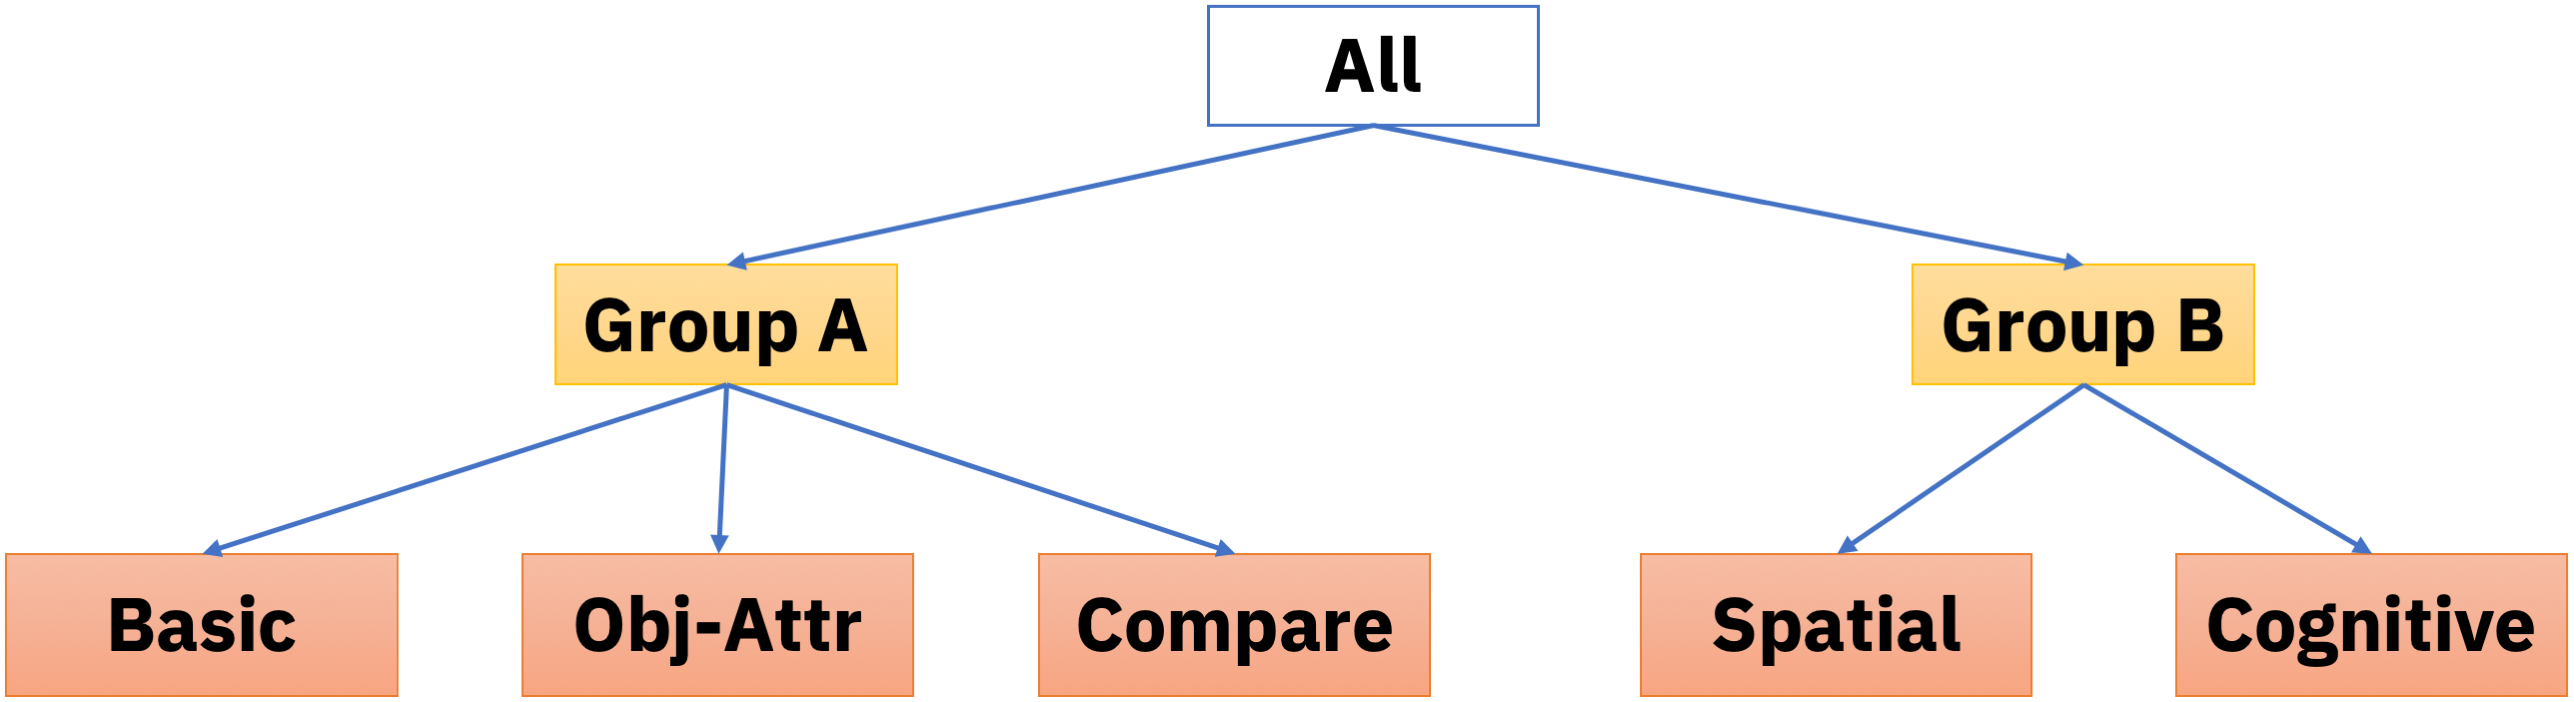
\includegraphics[width=\columnwidth]{../img/architecture/hierarchy}
	\caption{Hierarchy of Task Groups.}
	\label{fig:task-groups}
\end{figure}

For groups at the lowest level, we chose the following task classes to be placed in those groups.
Below, substitute each of \textit{Shape} and \textit{Color} for  \uX{} to obtain the task class.
\begin{description}
	\compresslist
	\item[Basic:] \textit{Exist}\uX, \textit{Get}\uX{} and \textit{Exist};
	\item[Obj-Attr:] \emph{SimpleCompare}\uX{} and \textit{AndSimpleCompare}\uX;
	\item[Compare:] \textit{Compare}\uX,  \textit{AndCompare}\uX{} \& \textit{Exist}\uX\textit{Of};
	\item[Spatial:] \textit{ExistSpace}, \textit{Exist}\uX\textit{Space}, and \textit{Get}\uX\textit{Space};
	\item[Cognitive:] \textit{ExistLastColorSameShape}, \textit{ExistLastShapeSameColor} and \textit{ExistLastObjectSameObject}
\end{description}


\tk{comparison of our model with baseline - pure COG, no transfer learning}
\tk{figure 3 from the orig paper}

baseline model~\cite{yang2018dataset}

We trained SAMNet using 8 reasoning steps (k=8) and external memory of 8 address locations, each storing an array of 128 floats. 
%We have also carried out experiments with different numbers of reasoning steps and memory size, but this goes beyond the scope of this paper.
We compared our results with the baseline model introduced in the same paper as the COG dataset~\cite{yang2018dataset}.
The most important results are highlighted in~\cref{fig:samnet_cog_detailed}; full comparison can be found in the supplementary material.%Appendix~\ref{sec:cog-all-results}.

\tk{comparison with results from softpahts?}


\newpage
\subsection{Feature transfer on CLEVR-CoGenT}

\tk{comparison of our model with baselines - CoGenT}
\tk{figure 3 from the orig paper}


\begin{figure}[htbp]
	\centering
	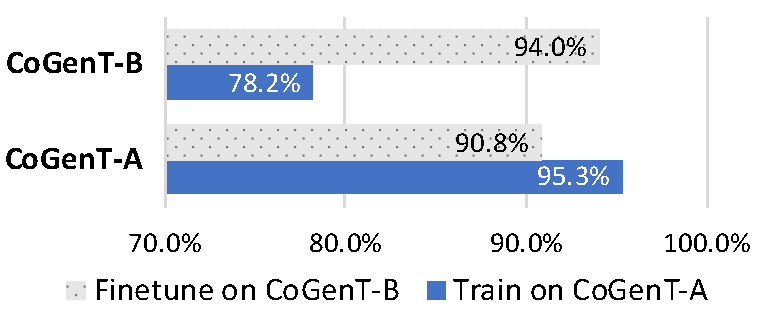
\includegraphics[width=0.8\columnwidth]{../results/CoGenT_B_results.pdf}
	\caption{Test accuracy on CoGenT-A \& -B when training on CoGenT-A (blue) and fine-tuning on CoGenT-B (gray).}
	\label{fig:CoGenT-B-results}
\end{figure}




\newpage
\subsection{Temporal transfer in COG}
\label{sec:temporal}

The goal here is to test the transfer learning ability concerning the frame sequence length, frame history required
for reasoning, and the number of object distractors.
For that purpose, we compare both models when trained on the Canonical variant but tested on the 
Hard variant (\cref{fig:samnet_cog_overall_transfer}).
The light gray color indicates original accuracies of the baseline model from paper, 
whereas dark gray indicates accuracies of the baseline model
obtained by running the original code provided by the authors~\cite{yang2018implement}.

The first column displays the scores of the traditional ML setup when training and testing on the Canonical variant. 
The observed close scores in light and dark gray underscore the baseline model reproducibility.
For both cases of zero-shot learning (second column--91.6\% vs 65.9\%) and fine-tuning using a single epoch 
(third column--96.7\% vs. 78.1\%), SAMNET outperforms the baseline model significantly.
Interestingly, this fine-tuning yields a mild boost of +0.6\% on the earlier reported accuracy 
in~\cref{sec:cog-baseline-compare} (fourth column).
These results suggest that it suffices to train SAMNet on simpler videos 
to enable learning of good memory usage and attention on relevant entities  
in order to achieve comparable, if not better, 
performance on longer video frames with more complex scenes.

\begin{figure}[htbp]
	\centering
	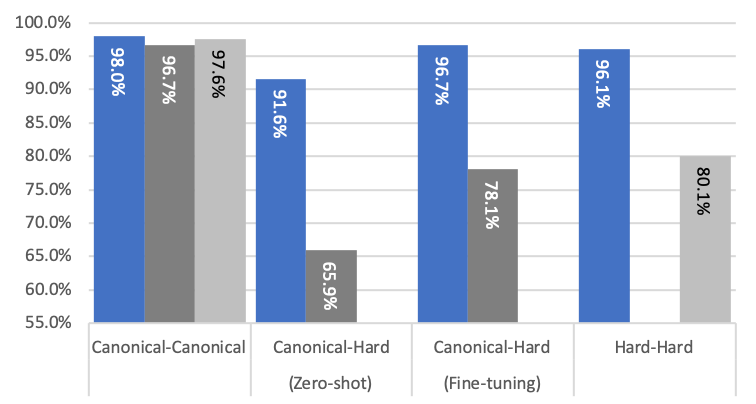
\includegraphics[width=\columnwidth]{../results/samnet_cog_overall_transfer.png}
	\caption{Total accuracies of SAMNet (blue) and baseline models (light/dark gray) when testing generalization from Canonical to Hard variants of the dataset.}
	\label{fig:samnet_cog_overall_transfer}
\end{figure}


\newpage
\subsection{Reasoning transfer on CLEVR-CoGenT}

\begin{figure}[htbp]
	\centering
	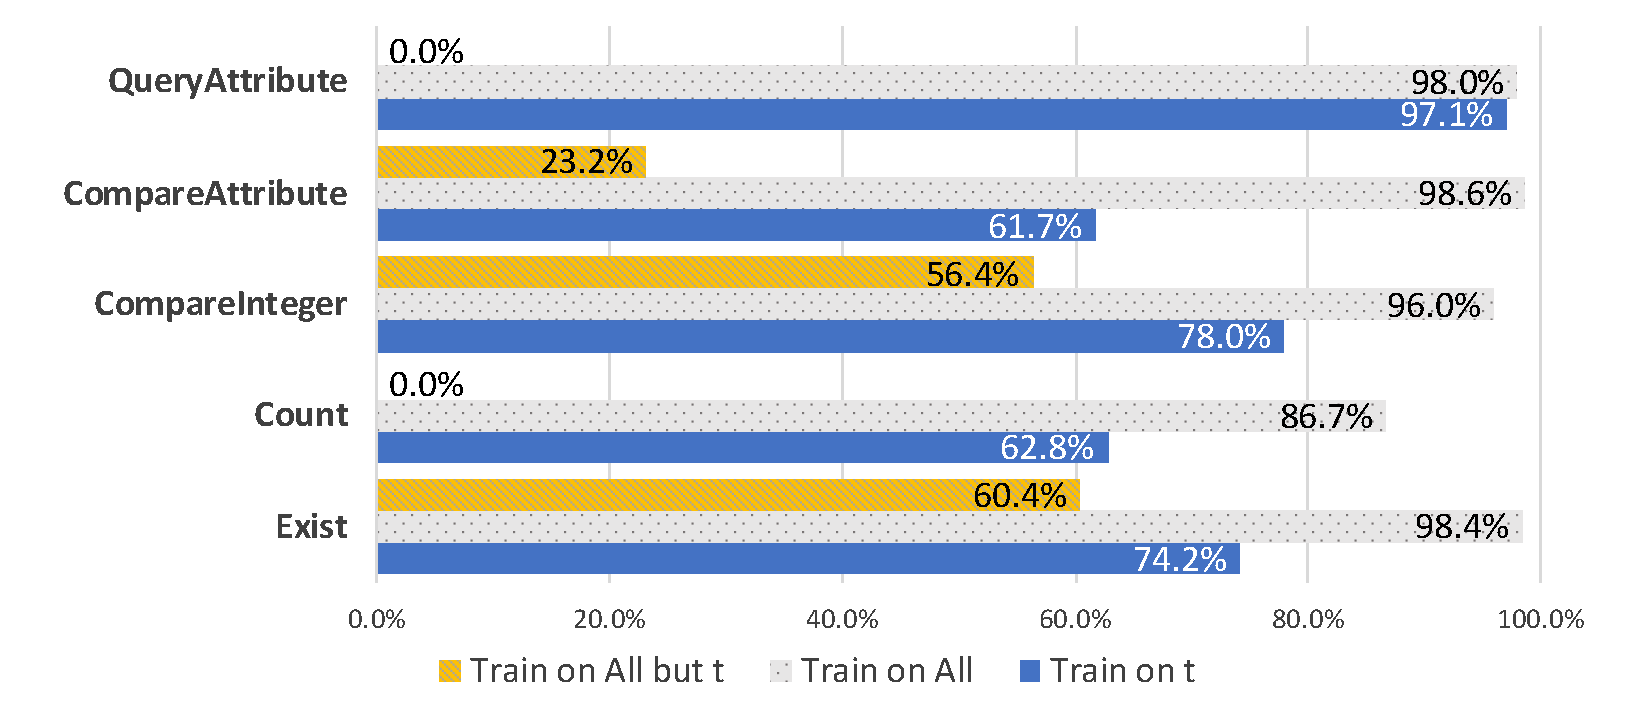
\includegraphics[width=\columnwidth]{../results/CoGenT_results.pdf}
	\caption{CLEVR-CoGenT accuracies for all tasks $t$ when training on $t$ only, training on all tasks jointly and training on all tasks but $t$.} %For all experiments, the validation and test sets are identical.
	\label{fig:CoGenT-results}
\end{figure}



\newpage
\subsubsection{Reasoning transfer on COG}


\begin{figure}[htbp]
	\centering
	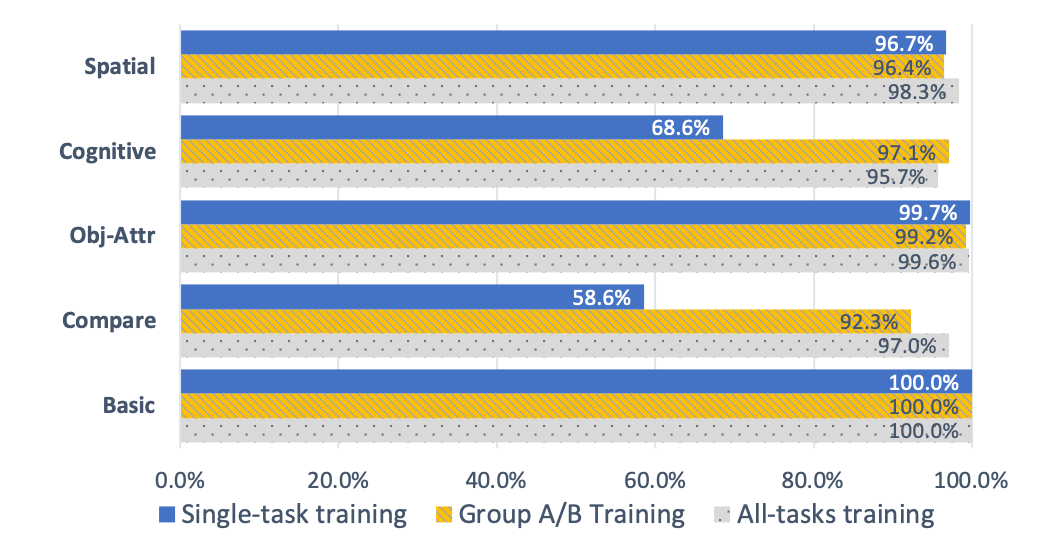
\includegraphics[width=\columnwidth]{../results/COG_reasoning_transfer_v3}
	\caption{COG accuracies for all task groups $t$ when training on $t$ only; training on Group A or B; and on all tasks.}
	\label{fig:COG-reasoning-results}
\end{figure}



